During this second year another four territorial PoPs have been raised and made operative, amounting to a total of eight territorial and the concentration one (Telvent -Barcelona) operational. Figure~\ref{fig:pop_weathermap} shows their distribution on the map. So far all the territorial PoPs are connected to the concentration one via XOC connections\footnote{The prices can be found at \url{http://www.xarxaoberta.cat/en/prices}.}.

\begin{figure}[H]
  \centering
  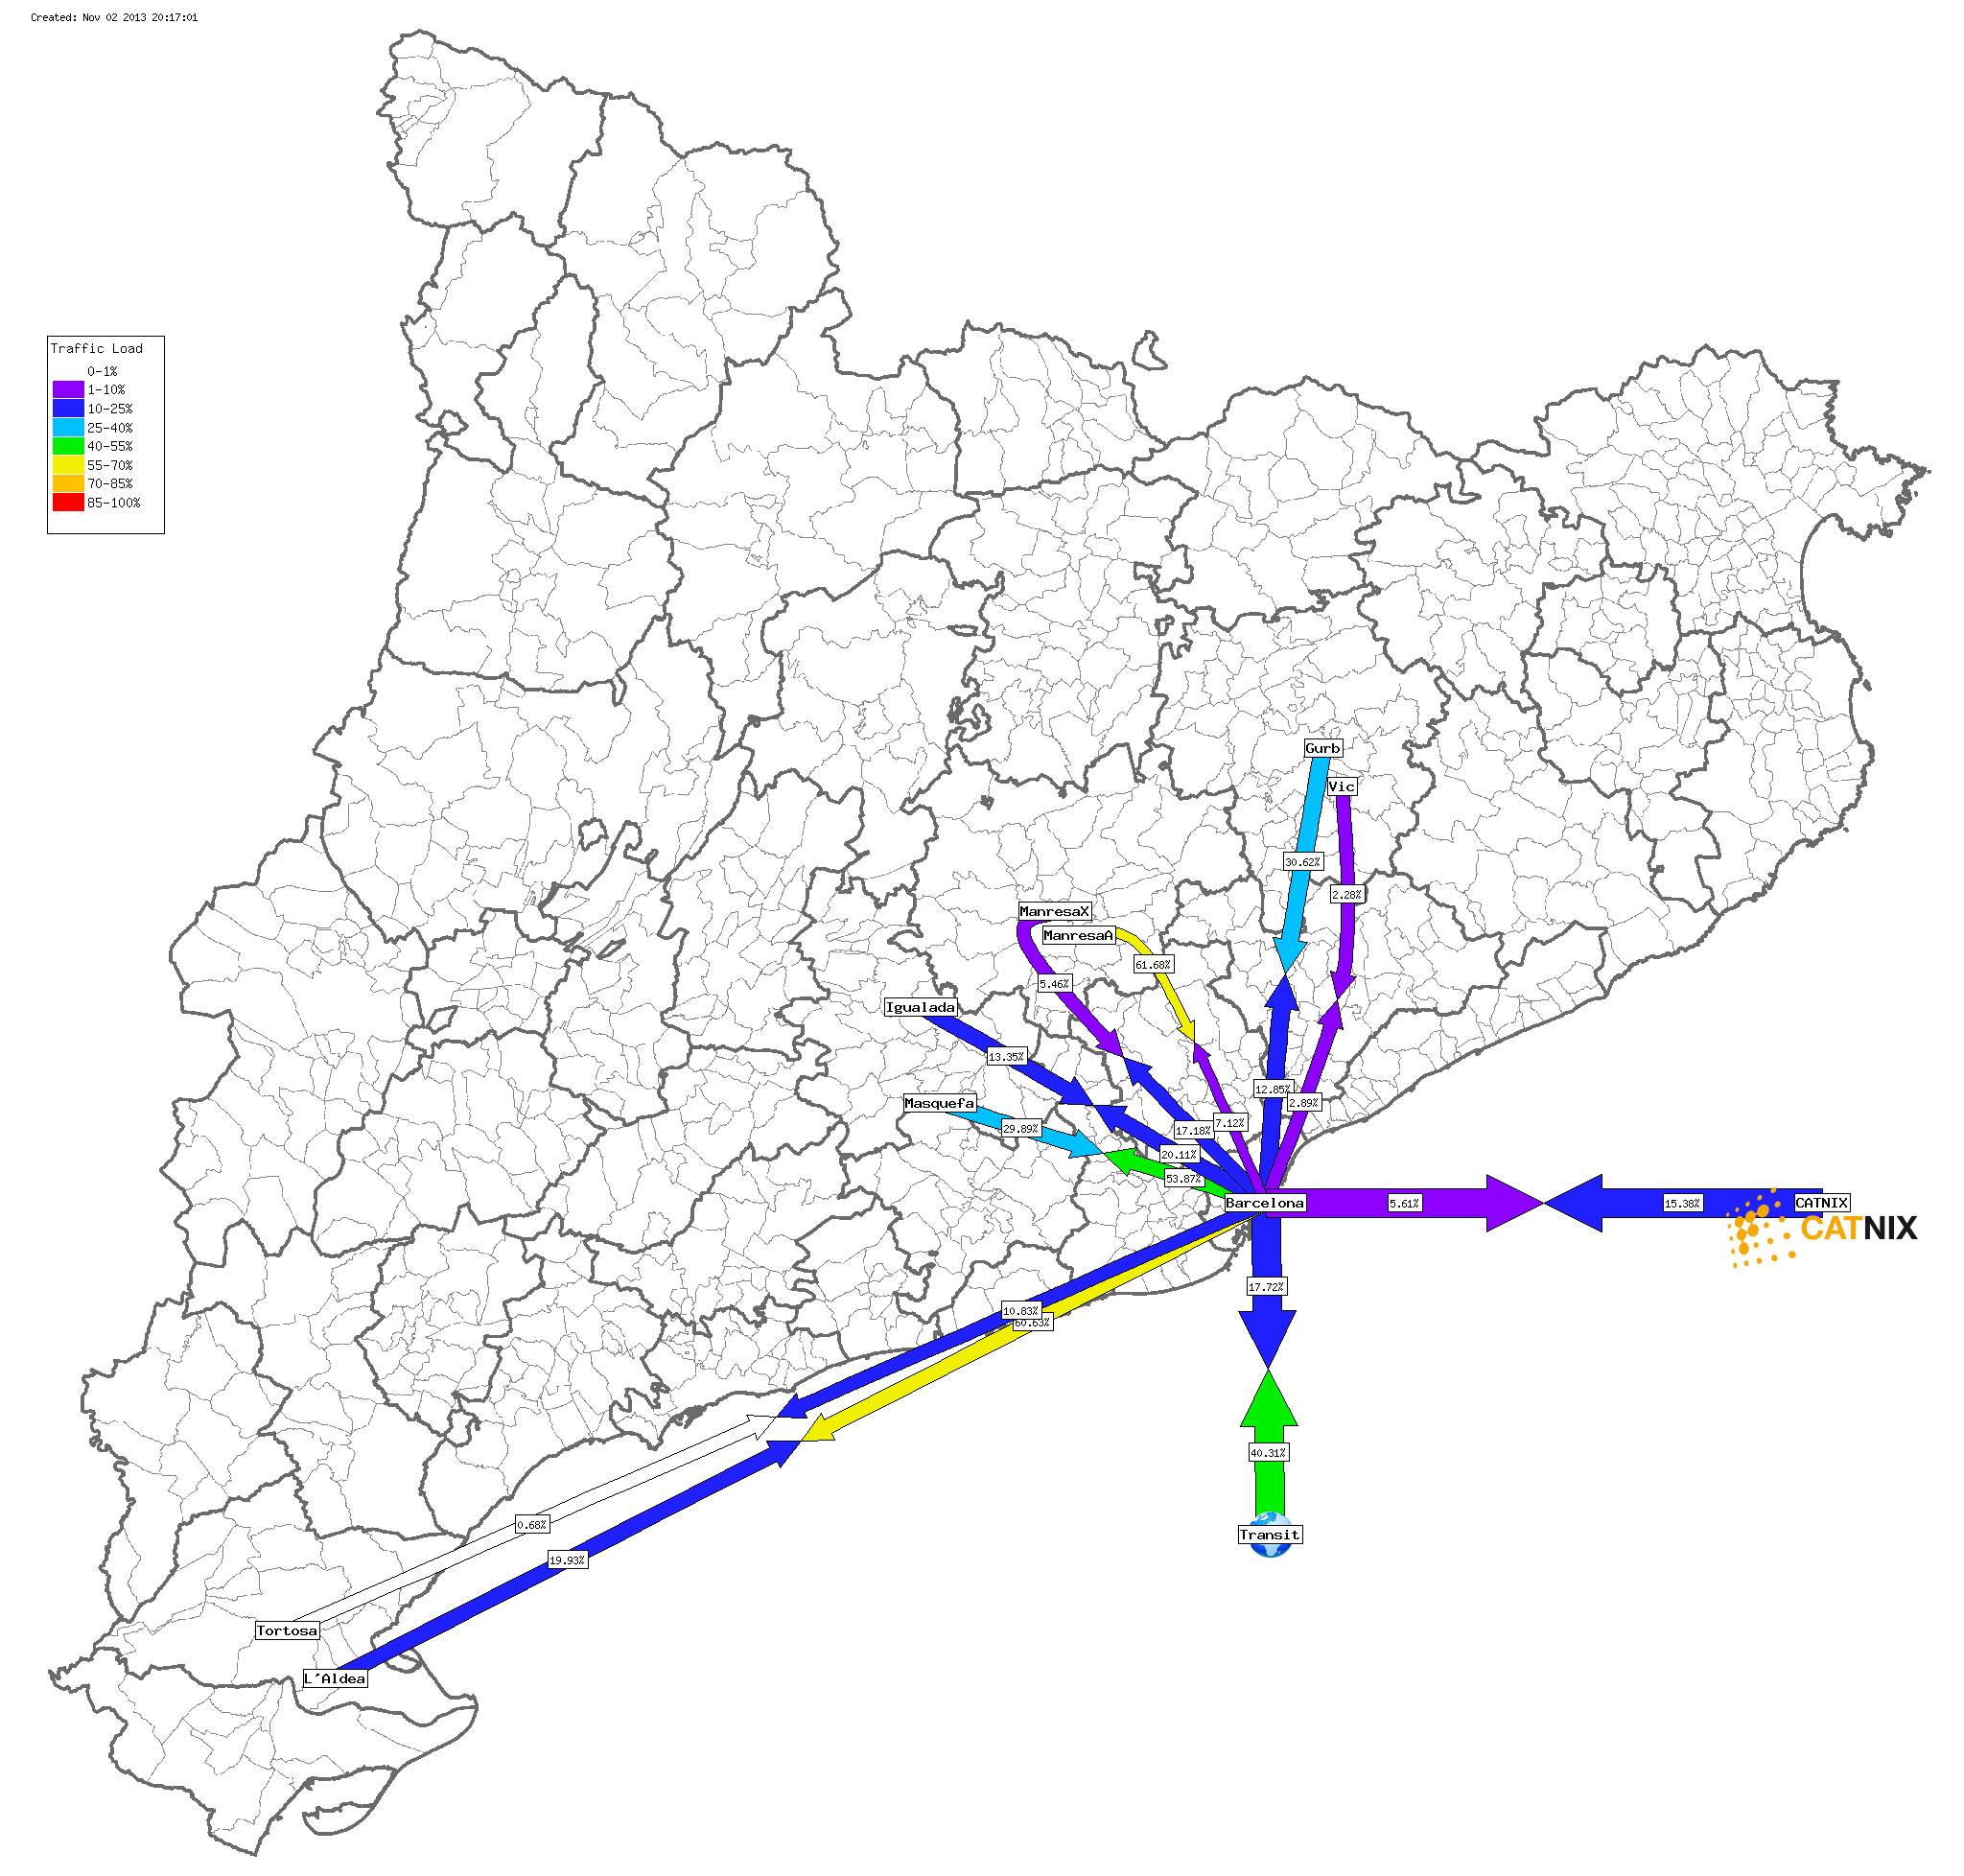
\includegraphics[width=0.95\linewidth]{sect3/figures/weathermap.png} 
  \caption[Guifi.net fiber POPs network map 2013]{Guifi.net fiber POPs network map 2013.}
  \label{fig:pop_weathermap}
\end{figure}

With respect to the IXs operation, the following improvements have been applied during this year:
\begin{itemize}
  \item The management system has been notably enhanced.
  \item A new monitoring development was launched in June 2013 (consequently, most of the traffic graphs shown in the document stars at that moment).
  \item The implementation of a more efficient accounting system has been started and it is expected to be fully operational in 2014. This system will make the ISPs' theshowback/chargeback more accurate and fair.
  \item The equipment of most of the PoPs has been completed and updated.
\end{itemize}

As an example of the current state of the art of the PoPs Figure~\ref{fig:telvent_diagram} shows Telvent's PoP at wiring level.

\begin{figure}[H]
  \centering
  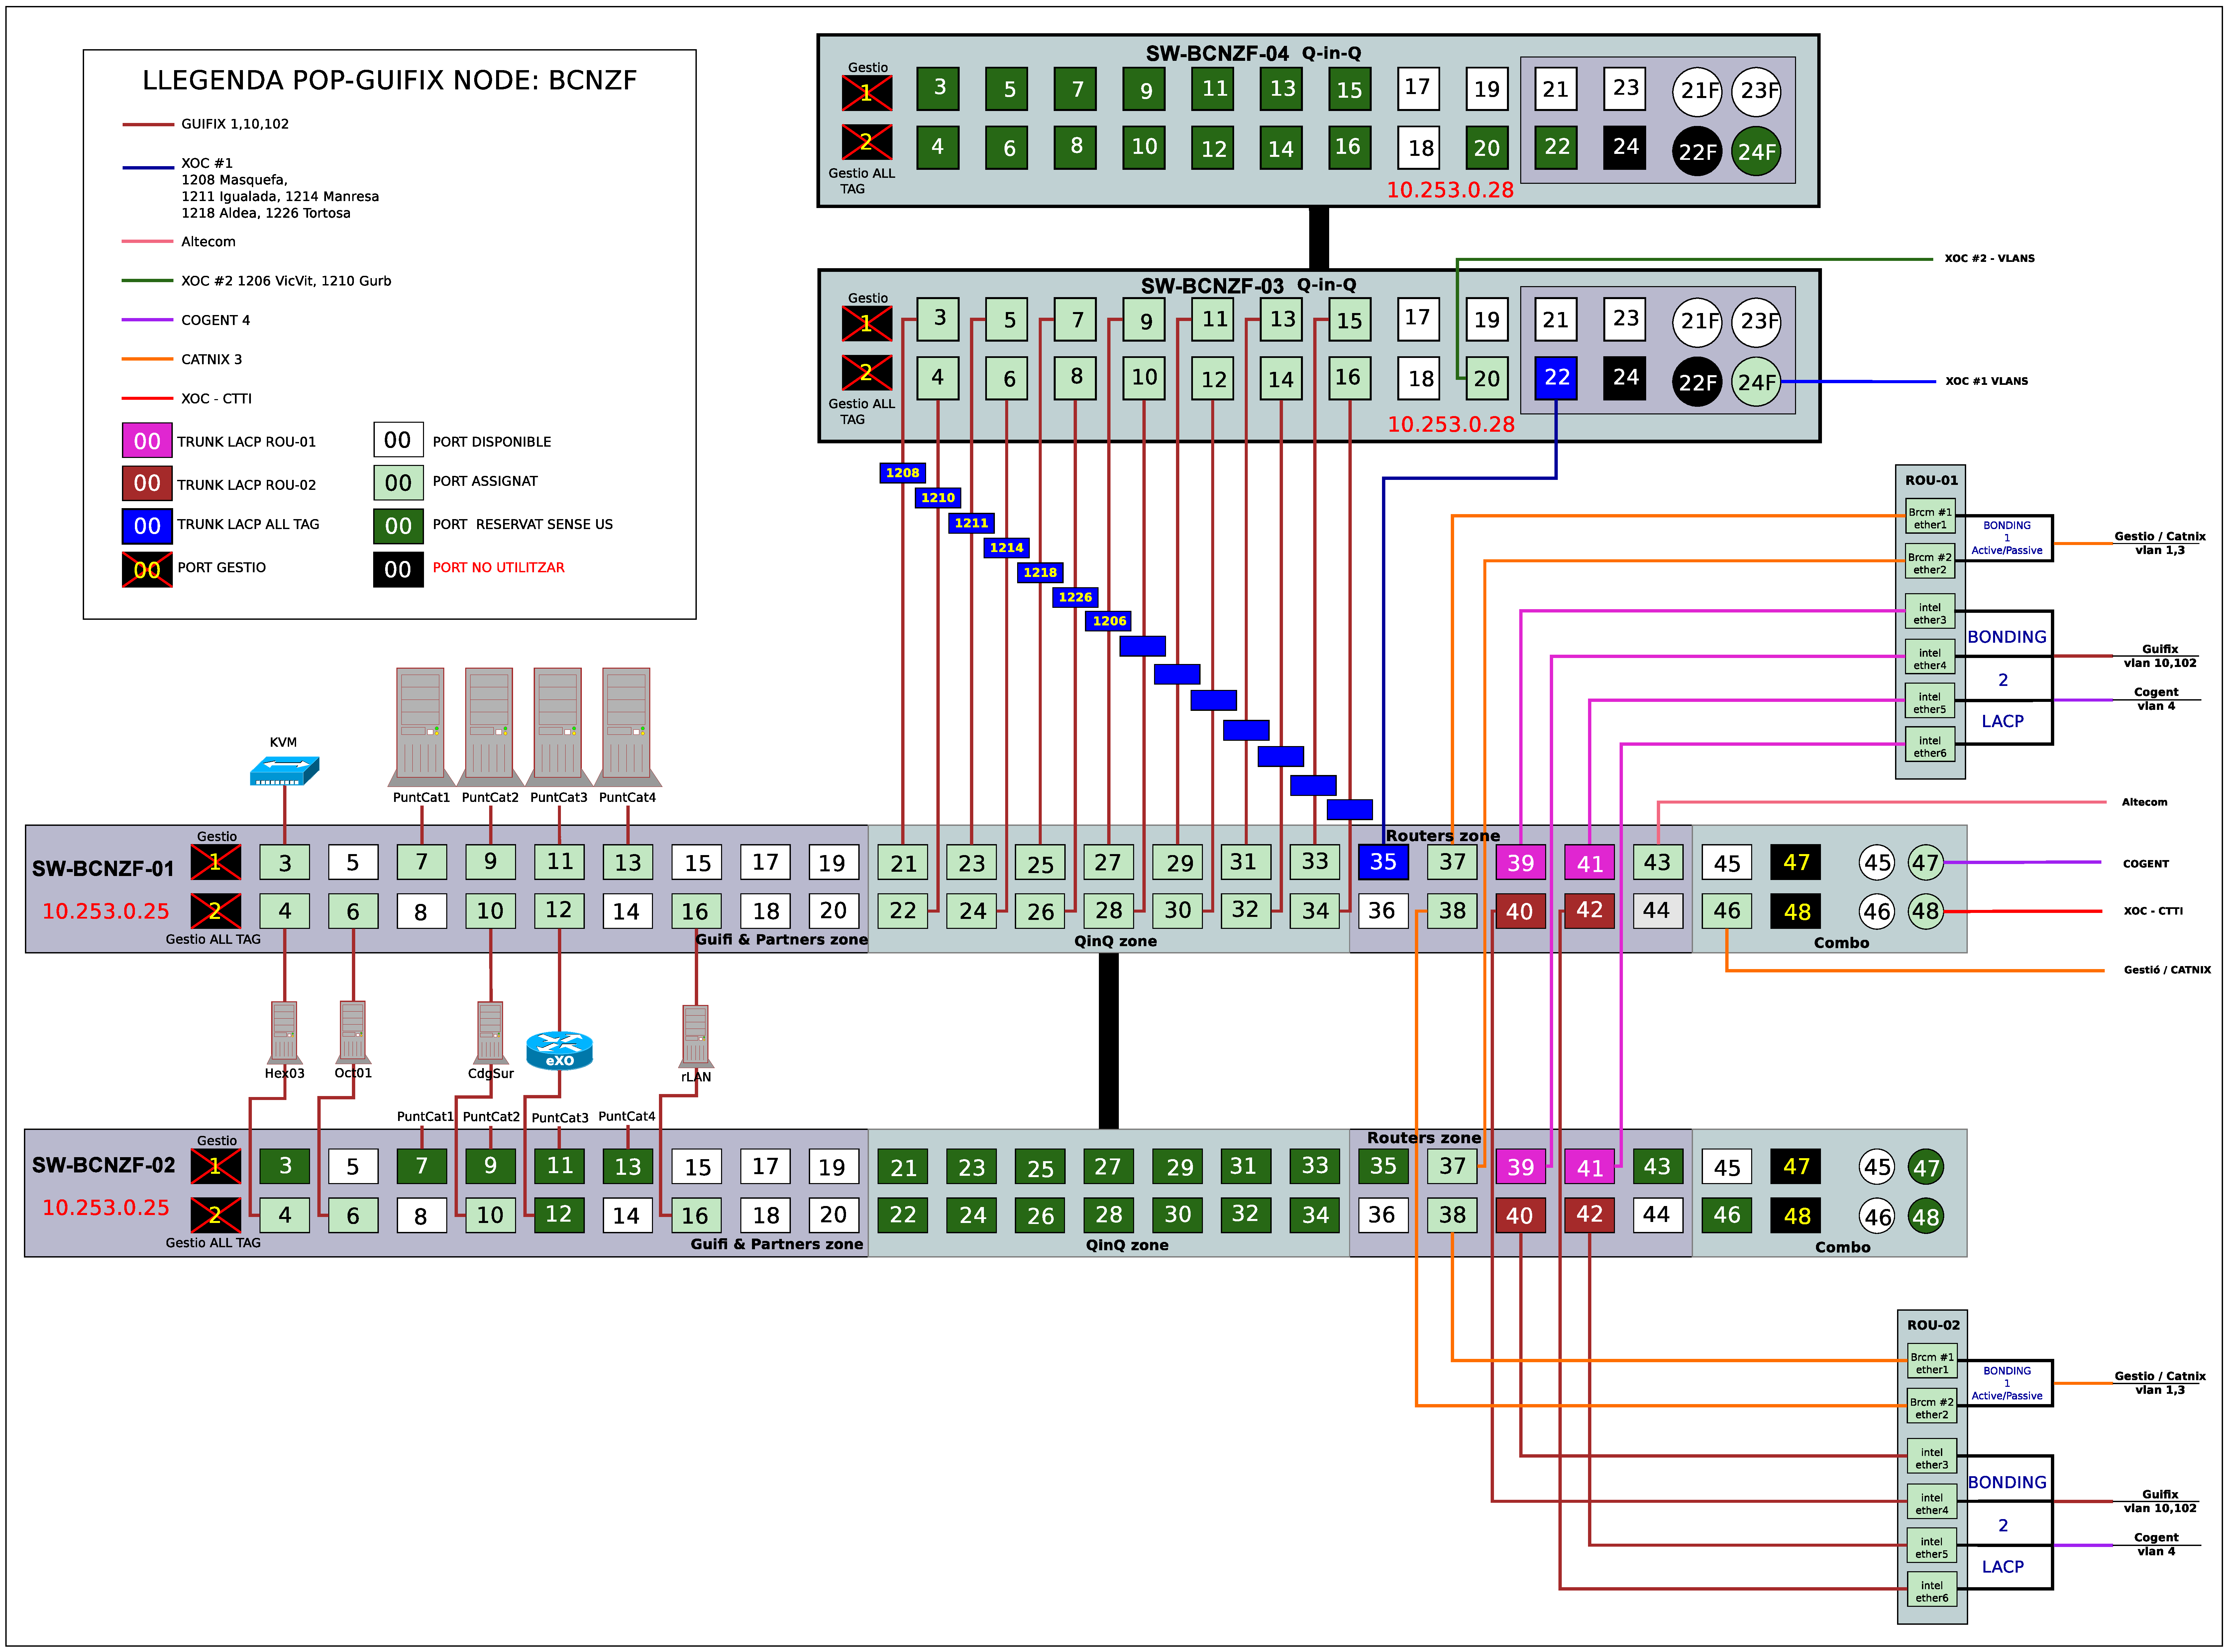
\includegraphics[width=0.95\linewidth]{sect3/figures/telvent_diagram.eps} 
  \caption[Telvent network diagram]{Telvent network diagram Oct. 2013.}
  \label{fig:telvent_diagram}
\end{figure}


During this period the CATNIX (the Catalan exchange point) peering process has been completed. As a result, the guifi.net Foundation is peering with all the other CATNIX members with the exception of the big ISPs (the Telefonica -the incumbent, Ono and BT). These ISPs have not shown any interest in peering with us.

Figure~\ref{fig:catnix_transit} shows the evolution of the peering traffic and Figure~\ref{fig:cogent_transit} shows the traffic to Cogent (our internet carrier). A second carrier is expected to be hired in the coming weeks, essentially to have a redundant internet access but also to anticipate the bandwidth demand.

\begin{figure}[H]
  \centering
  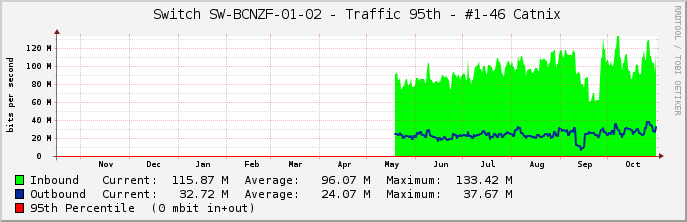
\includegraphics[width=0.95\linewidth]{sect3/figures/catnix.png} 
  \caption[CATNIX traffic 2013]{CATNIX traffic 2013.}
  \label{fig:catnix_transit}
\end{figure}

\begin{figure}[H]
  \centering
  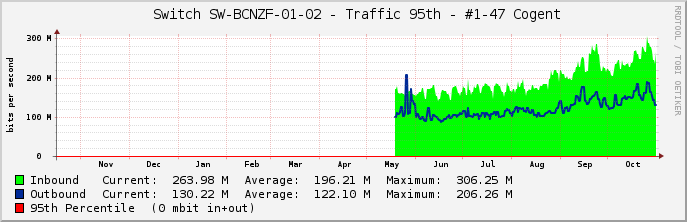
\includegraphics[width=0.95\linewidth]{sect3/figures/cogent.png} 
  \caption[Cogent traffic 2013]{Cogent traffic 2013.}
  \label{fig:cogent_transit}
\end{figure}

\FloatBarrier
\subsection{Pilot's POPs}
\label{pop_pilots}


\FloatBarrier
\subsubsection{Gurb}
\label{pop_gurb}

This PoP has been operative since 2010. This year the power supply system has been improved by adding a back-up power supply. Also the electronic equipment has been significantly extended to accommodate the necessities deriving from Gurb's OF pilot deployment and other connections. Firgure~\ref{fig:gurb_transit} shows the transit of this PoP.

\begin{figure}[H]
  \centering
  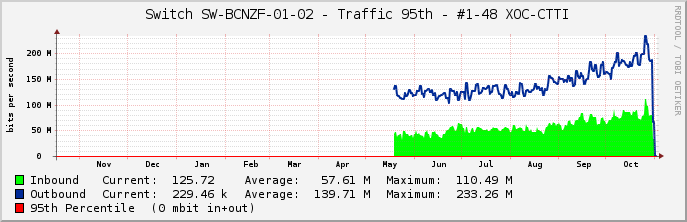
\includegraphics[width=0.95\linewidth]{sect3/figures/gurb.png} 
  \caption[Gurb PoP traffic 2013]{Gurb PoP traffic 2013.}
  \label{fig:gurb_transit}
\end{figure}


\FloatBarrier
\subsubsection{Vic}
\label{pop_vic}

As already foreseen in the previous report, this PoP was activated few days after the report was realised. Despite the fact that Vic borders Gurb, This PoP was raised as an alternative to the impossibility of reaching the Gurb's PoP. The equipment is allocated in a data centre of a facilitate of the local government (http://www.vitvic.cat/). Firgure~\ref{fig:vic_transit} shows the transit of this PoP.

\begin{figure}[H]
  \centering
  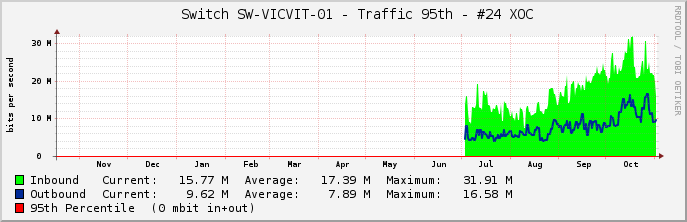
\includegraphics[width=0.95\linewidth]{sect3/figures/vic.png} 
  \caption[Vic PoP traffic 2013]{Vic PoP traffic 2013.}
  \label{fig:vic_transit}
\end{figure}


\FloatBarrier
\subsubsection{Rub\'{i}}
\label{pop_rubi}

In contrast to Vic, where due to its proximity to Gurb the option of not raising a PoP was worked, Rubí pilot clearly needs its own PoP. Thus, if the pilot is eventually developed in 2014 this PoP must be raised.


\FloatBarrier
\subsection{Other POPs}
\label{pop_others}

Firgure~\ref{fig:others_transit} shows the transit of the rest of the operational territorial PoPs .


\begin{figure}[H]
  \centering
    \begin{tabular}{c}
      \resizebox{0.75\linewidth}{!}{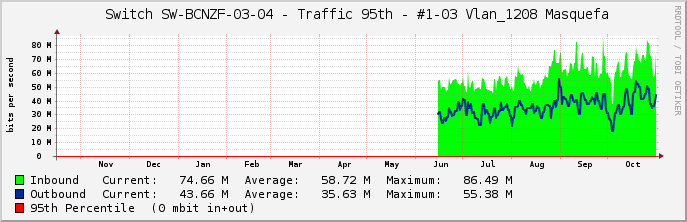
\includegraphics{sect3/figures/masquefa.png}} \\
      \resizebox{0.75\linewidth}{!}{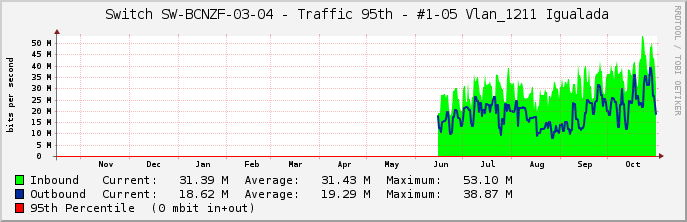
\includegraphics{sect3/figures/igualada.png}} \\
      \resizebox{0.75\linewidth}{!}{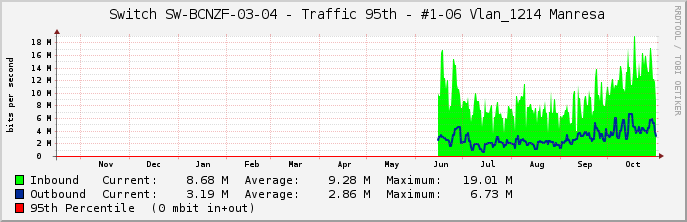
\includegraphics{sect3/figures/manresa.png}} \\
      \resizebox{0.75\linewidth}{!}{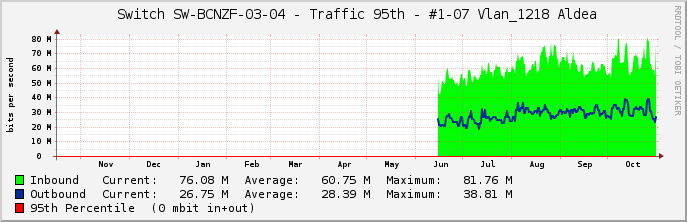
\includegraphics{sect3/figures/aldea.png}} \\
      \resizebox{0.75\linewidth}{!}{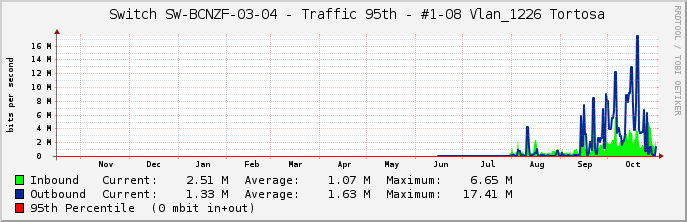
\includegraphics{sect3/figures/tortosa.png}} \\
    \end{tabular}
  \caption[Other PoPs traffic 2013]{Other PoPs traffic 2013. Top: Masquefa. Second top: Igualda. Middle: Manresa. Second bottom: Aldea. Bottom: Tortosa.}
  \label{fig:others_transit}
\end{figure}

%\item Masquefa
%\item Igualda
%\item Manresa
%\item Aldea
%\item Tortosa
